\section{Genetic Algorithm}
\label{sec:ea}

A genetic algorithm (GA) is a population-based metaheuristic optimization algorithm that is based on Darwin's theory of natural evolution. Darwin theorized that over a period of time a population of individuals would naturally mate and create offspring that were better than themselves. He suggested that not all individuals are created equally and that eventually the weaker individuals would die off. This same principle can be applied to a search algorithm as a heuristic. A GA contains a population of individuals that are evolved to find improved candidate solutions.

Figure~\ref{fig:evolutionaryFlowchart} demonstrates how the basic GA operates. Initially a \textit{population} of candidate solutions is generated. The individuals are evaluated based on an \textit{evaluation function} and are checked against the \textit{stopping criterion}. If the \textit{stopping criterion} has not been reached the population goes through an \textit{evolutionary period} where a new population of candidate individuals are created from the last population. This iterative process, also called a \textit{generation}, is repeated until the \textit{stopping criterion} is reached. The following subsections will explain each of these parts.

\begin{figure}[H]
	\centering
	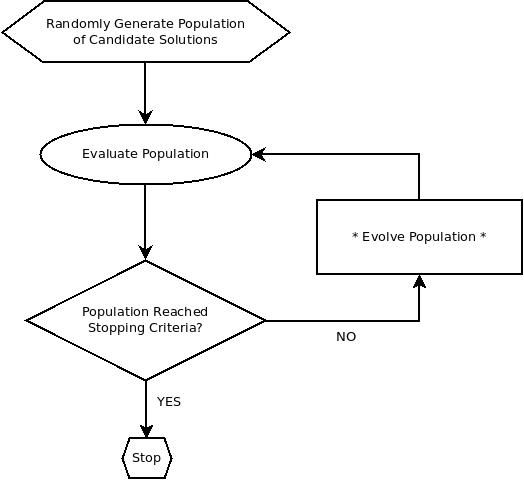
\includegraphics[bb=0 0 524 481,scale=0.5]{figures/EA.jpeg}
	\caption{Basic GA Flowchart}
	\label{fig:evolutionaryFlowchart}
\end{figure}

\subsection{Population}

The population is a key piece to a GA. Each individual in the population represents a possible candidate solution to the problem that we are attemping to solve. The representation of the individual is usually unique to the problem. Generating the initial population can either be done randomly or by some procedural method. The goal of generating the initial population is to create a diverse enough population to find improved solutions.

During each generation a new population is created using the previous generation's population. Initially the best individuals from the previous population might be copied directly into the new population using an operator called \textit{elitism}. To obtain the remaining individuals needed to fill the new population a \textit{selection} process occurs. Two individuals are chosen using a \textit{selection} method and then one of three options can occur: \textit{crossover}, \textit{mutation}, or \textit{replication}. Crossover mixes two individuals together to create two new individuals, mutation randomly modifies each individual separately, and replication copies the individuals. The two individuals are then placed in the new population and the process is repeated until the new population is the same size as the previous population. Figure~\ref{fig:gaFlowchart} depicts how evolution occurs in a GA. See Subsection~\ref{subsec:ga-operators} for more details on the operators discussed.

\begin{figure}[H]
	\centering
	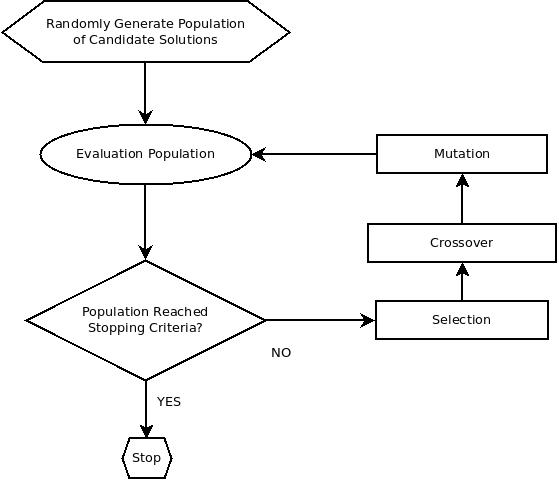
\includegraphics[bb=0 0 288 390,scale=0.5]{figures/GA.jpeg}
	\caption{GA Evolution}
	\label{fig:gaFlowchart}
\end{figure}

\subsection{Evaluation Function}
\label{subsec:fitness-function}

This operator determines the fitness of an individual. Each individual is evaluated and given a fitness score to represent how well the individual performed on the problem. This operation is problem specific and it can be very difficult to determine how a problem should be evaluated. The evaluation function is important for differentiating individuals. A poor evaluation function can make each of the individuals appear to be similar when they actually have small key differences. 

\subsection{Stopping Criterion}

Stopping criteria are used to determine when the GA should stop evolving. There are generally three ways stopping criteria can be reached: a maximum number of iterations is reached, the population has converged on the same solution, or the solution has been found.

\subsection{Genetic Operators}
\label{subsec:ga-operators}

Each of the following operators represent a piece of a genetic algorithm. They facilitate the evolutionary process in the effort to find better candidate solutions. Each of these operators has a unique purpose in the search algorithm but there are many different ways in which these goals can be carried out. Only a few of the different methods will be described in this work.

\textit{Selection Operator}: The idea behind this operator is to put selection pressure on the population during the evolutionary process. Individuals with a better fitness score should be allowed a better chance of continuing on to the next population. During the selection process two individuals are chosen using a selection method and then are either bred together, mutated, or replicated and placed in the next population. There are several varieties of selection methods but only \textit{k-Tournament selection} will be explained as this is the only method used in this work.

The \textit{k}-Tournament selection method works by randomly selecting \textit{k} individuals from the population, where \textit{k} is less than the number of individuals in the population, and selecting the individual that has the best fitness score from the \textit{k} individuals. The value of \textit{k} should be relatively small compared to the size of the population. If the value of \textit{k} is too large it would defeat the purpose of this selection method. For example, if there is a population size of 100 then a suitable value of \textit{k} is around 2-5.

\textit{Crossover Operator}: This operator is essential to evolving the individuals of the population. Crossover is the mechanism by which two individuals breed to create two new individuals. With respect to the evolutionary process, crossover exploits the current information that is contained within the population in order to find improved individuals. The most widely used type of crossover is N-point crossover.

N-point crossover works by randomly selecting N cutting points and swapping the information between the two individuals along those N points. Figure~\ref{fig:2PointCrossover} demonstrates how the swapping of information occurs during 2-point crossover.

\begin{figure}[H]
  \centering
  \begin{tabu}{ | p{1.5cm} | l | l |[2pt] l | l | l |[2pt] l | l | l | }
    \hline
    Parent 1 & \textcolor{blue}{0} & \textcolor{blue}{1} & \textcolor{blue}{1} & \textcolor{blue}{0} & \textcolor{blue}{1} & \textcolor{blue}{0} & \textcolor{blue}{1} & \textcolor{blue}{0} \\ \hline
    Parent 2 & \textcolor{red}{0} & \textcolor{red}{0} & \textcolor{red}{1} & \textcolor{red}{0} & \textcolor{red}{0} & \textcolor{red}{1} & \textcolor{red}{0} & \textcolor{red}{0} \\ \hline
  \end{tabu}
  \\
  \vspace{3 mm}
  \line(1,0){250}
  \\
  \vspace{3 mm}
  \begin{tabu}{ | p{1.5cm} | l | l |[2pt] l | l | l |[2pt] l | l | l | }
    \hline
    Child 1 & \textcolor{red}{0} & \textcolor{red}{0} & \textcolor{blue}{1} & \textcolor{blue}{0} & \textcolor{blue}{1} & \textcolor{red}{1} & \textcolor{red}{0} & \textcolor{red}{0} \\ \hline
    Child 2 & \textcolor{blue}{0} & \textcolor{blue}{1} & \textcolor{red}{1} & \textcolor{red}{0} & \textcolor{red}{0} & \textcolor{blue}{0} & \textcolor{blue}{1} & \textcolor{blue}{0} \\ \hline
  \end{tabu}
  \caption{2-Point Crossover}
  \label{fig:2PointCrossover}
\end{figure}

\textit{Mutation Operator}: The mutation operator is used to introduce random changes to the individuals during evolution. Mutations to individuals are a way to explore the search space. Depending on how the initial population was created there may not be the necessary information in the population to find the optimal solution with crossover alone. Mutations allow for new information to possibly be introduced into the population. A common type of mutation is single-point mutation where a single index in a given individual is modified. Figure~\ref{fig:mutation} demonstrates single-point mutation.

\begin{figure}[H]
  \centering
  \begin{tabular}{ | p{2cm} | l | l | l | l | l | l | l | l | }
    \hline
    Individual & 0 & 1 & 1 & 0 & 1 & 0 & 1 & 0 \\
    \hline
  \end{tabular}
  \\
  \vspace{3 mm}
  \line(1,0){250}
  \\
  \vspace{3 mm}
  \begin{tabular}{ | p{2cm} | l | l | l | l | l | l | l | l | }
    \hline
    Mutant & 0 & 1 & 1 & \textcolor{red}{1} & 1 & 0 & 1 & 0 \\
    \hline
  \end{tabular}
  \caption{Single-point Mutation}
  \label{fig:mutation}
\end{figure}

\textit{Elitism Operator}: During each generation of the genetic algorithm a new population is created using the individuals from the population in the previous generation. The new population is bred from the previous individuals with the hopes of creating better individuals. Sometimes this is not the case and the population can end up losing valuable information from individuals that were not chosen during the selection process. To prevent this from happening the elitism operator was created. The elitism operator works by seeding the next generation's population with the individuals with the best fitness score. Typically only the top 1\% of individuals are copied into the next generation.